\documentclass[tikz]{standalone}

\usepackage{amsmath}
\usepackage{physics}

\usetikzlibrary{arrows.meta,fit,positioning}

\begin{document}
	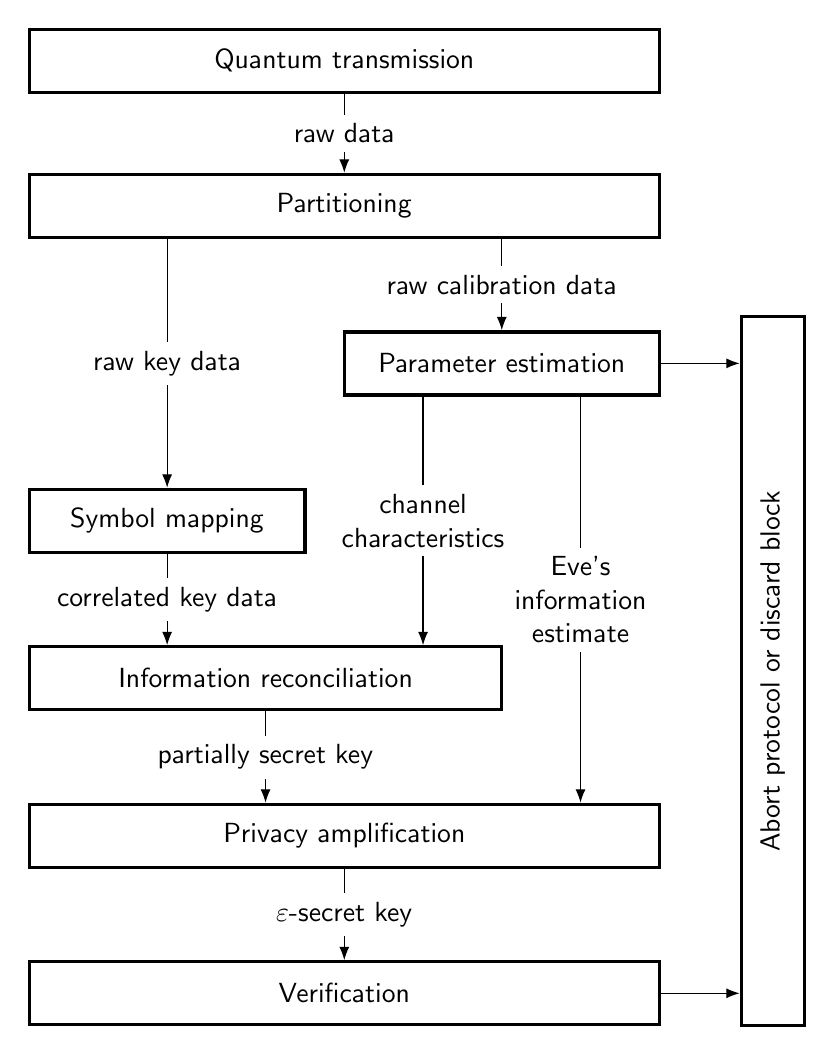
\begin{tikzpicture}[
		node distance=2cm,
		block/.style={draw, very thick, minimum height=0.8cm},
	]
		\node[block, minimum width=8cm] (qt) {\textsf{Quantum transmission}};
		\node[block, minimum width=8cm, below=1cm of qt] (pt) {\textsf{Partitioning}};		
		\node[block, below=of pt.east, anchor=east, minimum width=4cm] (pe) {\textsf{Parameter estimation}};
		\node[block, below=4cm of pt.west, anchor=west, minimum width=3.5cm] (sm) {\textsf{Symbol mapping}};
		\node[block, below=of sm.west, anchor=west, minimum width=6cm] (ir) {\textsf{Information reconciliation}};
		\node[block, below=of ir.west, anchor=west, minimum width=8cm] (pa) {\textsf{Privacy amplification}};
		\node[block, below=of pa.west, anchor=west, minimum width=8cm] (ver) {\textsf{Verification}};
		
		\draw[-Latex] (qt) -- (pt) node[midway, fill=white]{\textsf{raw data}};
		\draw[Latex-] (sm.north) -- (sm.north|-pt.south) node[midway, fill=white] {\textsf{raw key data}};
		\draw[Latex-] (pe.north) -- (pe.north|-pt.south) node[midway, fill=white] {\textsf{raw calibration data}};
		\draw[-Latex] (sm.south) -- (sm.south|-ir.north) node[midway, fill=white] {\textsf{correlated key data}};
		\draw[-Latex] (ir.south) -- (ir.south|-pa.north) node[midway, fill=white] {\textsf{partially secret key}};
		\draw[-Latex] (pa) -- (ver) node[midway, fill=white] {\textsf{$\varepsilon$-secret key}};
		\begin{scope}[transform canvas={xshift=-1cm}]
			\draw[-Latex] (pe.south) -- (pe.south|-ir.north) node[midway, fill=white, align=center]{\textsf{channel}\\\textsf{characteristics}};
		\end{scope}
		\begin{scope}[transform canvas={xshift=1cm}]
			\draw[-Latex] (pe.south) -- (pe.south|-pa.north) node[midway, fill=white, align=center]{\textsf{Eve's}\\\textsf{information}\\\textsf{estimate}};
		\end{scope}
		
		\node[block, right=1cm of qt, rotate=90, anchor=north, xshift=-7.75cm, minimum width=9cm] (abort) {\textsf{Abort protocol or discard block}};
		\draw[-Latex] (pe.east) -- (pe.east-|abort.north);
		\draw[-Latex] (ver.east) -- (ver.east-|abort.north);
	\end{tikzpicture}
\end{document}